\documentclass[a4paper, 12pt, titlepage]{article}

% Including needed packages
\usepackage[margin=2cm]{geometry}
\usepackage{amsmath}
\usepackage{amssymb}
\usepackage{graphicx}

\title
{{\em MAP 565 - Time series analysis}\\
Mini-project - Smoothing trajectories using Kalman filter\\
{\bf Report}}
\author{KLINTEFELT COLLET Philippe \and ROHRMANN Till}
\date{}

\begin{document}

\maketitle

\section{Question}

Given the position $P(t)$, velocity $V(t)$ and acceleration $A(t)$ of an object moving along a one dimensional axis. 
Furthermore, given the time discretization by $t_k=\delta k$ for $k\in \mathbb{Z}$.
The discretization quantities are denoted by $P_k=P(t_k)$, $V_k=V(t_k)$ and $A_k=A(t_k)$.
Assuming that $A(t)\approx A(t_{k-1})$ for $t\in (t_{k-1},t_k)$ for all $k\in\mathbb{Z}$ and that the discretization step $\delta$ is small.
Show that the following equations hold:
\begin{eqnarray}
	V_k &\approx& V_{k-1} + \delta A_{k-1}\\
	P_k &\approx& P_{k-1} + \delta V_{k-1} + \frac{\delta^2}{2} A_{k-1}
\end{eqnarray}

\paragraph{Proof}

Since $A(t)$ is the derivative of $V(t)$ it holds.
\begin{eqnarray}
	V(t_k) - V(t_{k-1}) &=& \int_{t_{k-1}}^{t_k} A(t)\ dt
\end{eqnarray}

By using the assumption of $A(t)\approx A(t_{k-1})$ for $t\in (t_{k-1},t_k)$ for all $k\in\mathbb{Z}$ we can transform the integral.
\begin{eqnarray}
	V_k &\approx& V_{k-1} + A_{k-1} \int_{t_{k-1}}^{t_k}\ dt \\
	&=& V_{k-1}+\delta A_{k-1}
\end{eqnarray}

The same reasoning holds for the position. 
Hence we obtain the following derivation.

\begin{eqnarray}
	P(t_k) - P(t_{k-1}) &=& \int_{t_{k-1}}^{t_k} V(t)\ dt\\
	P_k &=& P_{k-1} + \int_{t_{k-1}}^{t_k}\left( V_{t_{k-1}} + \int_{t_{k-1}}^{t} A(t^{\prime})\ dt^{\prime}\right)\ dt\\
	P_k &\approx& P_{k-1} + \delta V_{t_{k-1}} + \int_{t_{k-1}}^{t_k} A_{k-1}(t-t_{k-1})\ dt\\
	&=& P_{k-1} + \delta V_{t_{k-1}} + \frac{\delta^2}{2} A_{k-1}	
\end{eqnarray}

\section{Question}

The state vector is defined as following: $\pmb{X}_t=(P_{k,1},P_{k,2},A_{k,1},A_{k,2})^T$.
Assuming 
\begin{eqnarray}
	\pmb{X}_{k} &=& \Phi \pmb{X}_{k-1} + \Pi \pmb{A}_{k-1} \label{eq}\\
	\Phi &=& \left(
		\begin{array}{cccc}
			1 &0 & \delta & 0\\
			0 & 1& 0 & \delta\\
			0 & 0& 1& 0\\
			0 & 0& 0& 1
		\end{array}
	\right)\\
	\Pi &=& \left(
		\begin{array}{cc}
			\delta^2/2 & 0\\
			0 & \delta^2/2\\
			\delta& 0\\
			0 & \delta
		\end{array}
	\right)\\
	\pmb{A}_{k-1} &=& \left (
		\begin{array}{c}
			A_{k-1,1}\\
			A_{k-1,2}
		\end{array}
	\right)
\end{eqnarray}

\paragraph{What conditions must hold for the state-space to be modelled like that?}
This modelling is only correct if the velocity $V(t)$ equals the acceleration $A(t)$. 
This implies $V(t)=A(t)=\frac{dV}{dt}$ and consequently $V(t)=A(t)=Ce^t$ where $C$ is any constant.% It was ''$V(t)=A(t)=e^t$' but isn't ''$V(t)=A(t)=Ce^t$ where $C$ is any constant'' more accurate? Or is that too obvious/irrelevant?

\section{Question}

Assuming the state-space vector now as $\pmb{X}_t=(P_{k,1},P_{k,2},V_{k,1},V_{k,2})^T$.
Furthermore, assume the sequences $(A_{t,1})$ and $(A_{t,2})$ are uncorrelated white noises with variance $\sigma^2$.
The equation \eqref{eq} can now be transformed into: %Protip: Use \eqref{} instead of (\ref{}) : It yields the same result.
\begin{eqnarray}
	\pmb{X}_{k} &=& \Phi \pmb{X}_{k-1} + \pmb{W}_{k-1}\\
	\pmb{W}_{k} &\sim& \mathcal{N}(0,Q)\\
	Q&=& \left(
		\begin{array}{cccc}
		\delta^4/4& 0& \delta^3/2 & 0\\
		0 & \delta^4/4 & 0& \delta^3/2\\
		\delta^3/2 & 0& \delta^2 &0\\
		0 & \delta^3/2 & 0 & \delta^2
		\end{array}
	\right)\sigma^2
\end{eqnarray}

\section{Question}

The implementation can be found in the file kalman.m.
The whole program can be run by executing run.m.

\section{Question}

\paragraph{Testing}

The implemented algorithm was applied to the provided data. To obtain the results presented in Figure \ref{fig:1}, Figure \ref{fig:2} and Figure \ref{fig:3} we set $\delta=1$, $\sigma=0.2$, $\kappa=10$ and $\rho$ was estimated to have the value $\rho=4.9428$.

\begin{figure}
	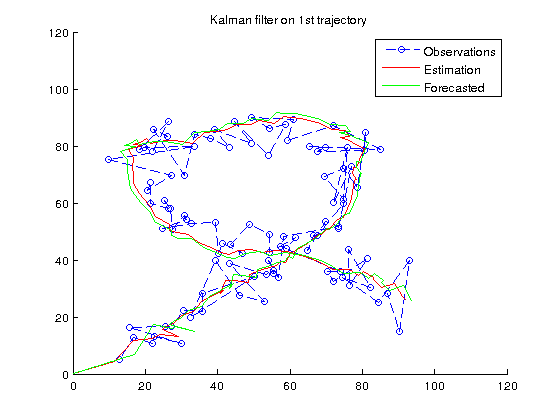
\includegraphics[width=15cm]{images/1trajectory.png}
	\caption{Kalman filter applied to first observation series. Blue circled-dashed line indicates the observations, red line the filtered estimation and green line the forecasted values.}
	\label{fig:1}
\end{figure}

\begin{figure}
	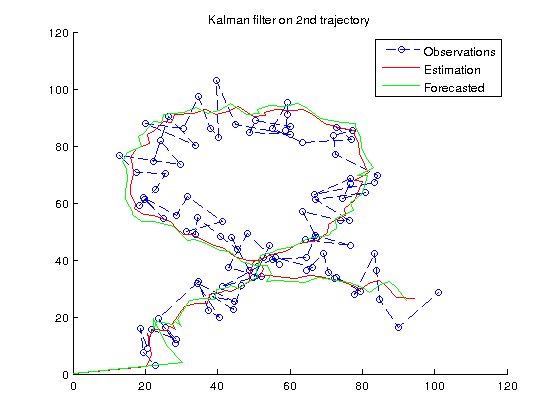
\includegraphics[width=15cm]{images/2trajectory.png}
	\caption{Kalman filter applied to second observation series. Blue circled-dashed line indicates the observations, red line the filtered estimation and green line the forecasted values.}
	\label{fig:2}
\end{figure}

\begin{figure}
	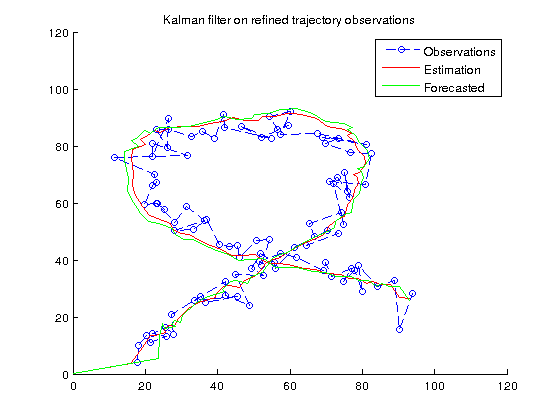
\includegraphics[width=15cm]{images/refinedTrajectory.png}
	\caption{Kalman filter applied to the refined observation series. Blue circled-dashed line indicates the observations, red line the filtered estimation and green line the forecasted values.}
	\label{fig:3}
\end{figure}

\paragraph{Estimating $\rho^2$}

For the observations the following equation holds:

\begin{eqnarray}
	\pmb{Y}_k &=& \Psi \pmb{X}_k + \pmb{V}_k \label{eqn:2}
\end{eqnarray}
where $\pmb{V}_k \sim \mathcal{N}(0,R)$ where $R=\rho^2\pmb{Id}_{2}$ and $\pmb{V}_k$ decorrelated from $\pmb{V}_j$ with $k\not=j$.
In order to estimate the parameter $\rho$ given to series of observations $\pmb{Y}$ and $\pmb{Y}^{\prime}$, we can calculate the difference and then use the ML-estimator for the variance of a Gaussian random variable.

\begin{eqnarray}
	\pmb{Y}_k - \pmb{Y}^{\prime}_k &=& \pmb{V}_k - \pmb{V}_{k}^{\prime} \label{eqn:1}
\end{eqnarray}

$\pmb{V}_k$ and $\pmb{V}^{\prime}_k$ are decorrelated (white noise) and since they are Gaussian variables they are also independent.
Therefore $\pmb{V}_k - \pmb{V}_{k}^{\prime}$ is also Gaussian distributed with $Var(\pmb{V}_k - \pmb{V}_{k}^{\prime}) = 2\ Var(\pmb{V}_k)$.
Since $\pmb{V}_{k,1}$ and $\pmb{V}_{k,2}$ are uncorrelated and thus independent we can consider each component as an independent realization of a Gaussian random variable with mean $\mu=0$ and variance $\sigma^2=\rho^2$.
Hence, $Var(\pmb{V}_{k,1} - \pmb{V}_{k,1}^{\prime}) = Var(\pmb{V}_{k,2} - \pmb{V}_{k,2}^{\prime}) =2\ \rho^2$.
By applying the ML-estimator for the variance of a Gaussian random variable
\begin{eqnarray}
	\hat{\sigma}^2 &=& \frac{1}{n-1}\sum_{i=1}^{n}(X_{i}-\hat{\mu})^2
\end{eqnarray}
we finally obtain our estimator of $\rho$.
\begin{eqnarray}
	2\ \hat{\rho}^2 &=& \frac{1}{2n-1}\left(\sum_{i=1}^{n}(\pmb{V}_{k,1} - \pmb{V}_{k,1}^{\prime})^2 + \sum_{i=1}^{n}(\pmb{V}_{k,2} - \pmb{V}_{k,2}^{\prime})^2 \right)
\end{eqnarray}


\paragraph{Initialization values}

In order to start the Kalman filter, initial values have to be provided to it.
If nothing is known about the starting position of the object, the first found evidence should be used.
That is to say, the estimation $\pmb{X}_{1\mid 1}$ of the position applied to the observation matrix should equal the first observation $\pmb{Y}_1$.

\begin{eqnarray}
	\pmb{X}_{1\mid 0} &=& \Phi \pmb{0} \\
	\pmb{X}_{1\mid 1} &=& \pmb{X}_{1\mid 0} + K_1(\pmb{Y}_1 -\Psi \pmb{X}_{1\mid 0})\\
	&=& \Sigma_{1\mid 0} \Psi^T \left[ \Psi\Sigma_{1\mid 0} \Psi^T +R \right]^{-1}\pmb{Y}_1\\
	\Psi\pmb{X}_{1\mid 1} &=& \Psi \Sigma_{1\mid 0} \Psi^T \left[ \Psi\Sigma_{1\mid 0} \Psi^T +R \right]^{-1}\pmb{Y}_1
\end{eqnarray}

By setting the initial value of the covariance matrix $\Sigma_0=\kappa^2 \pmb{Id}_4$, we obtain:

\begin{eqnarray}
	\Sigma_{1\mid 0} &=& \kappa^2\Phi \Phi^T + Q\\
	\Psi \Sigma_{1\mid 0} \Psi^T + R &=& \kappa^2 \Psi \Phi \Phi^T \Psi^T + \Psi Q \Psi^T + R
\end{eqnarray}

If $\kappa \gg \rho$ and $\kappa \gg \sigma$, then $\kappa^2 \Psi \Phi \Phi^T \Psi^T + \Psi Q \Psi^T + R \approx \kappa^2 \Psi \Phi \Phi^T \Psi^T$ and thus

\begin{eqnarray}
	\Psi\pmb{X}_{1\mid 1} &\approx& \Psi \Sigma_{1\mid 0} \Psi^T \left[ \Psi\Sigma_{1\mid 0} \Psi^T \right]^{-1}\pmb{Y}_1 = \pmb{Y}_1 
\end{eqnarray}

\paragraph{Influence of $\sigma^2$}

The value $\sigma^2$ influences how much effect the current observation with regard to the past observations has on the filtered estimation. 
That is to say, if the value $\sigma^2$ is high, the filtered estimation approaches the observations, whereas if the value is small, the past (average) observations determine more strongly the next filtered estimation value. 
This effect is illustrated in Figure \ref{fig:4} where the value of $\sigma^2=\frac{1}{100}$, Figure \ref{fig:5} where the value of $\sigma^2=1$ and Figure \ref{fig:6} where the value of $\sigma^2=100$. 
To conclude, the value of $\sigma^2$ determines the smoothness of the filtering. 
The lower its value, the smoother the filtering.

\begin{figure}
	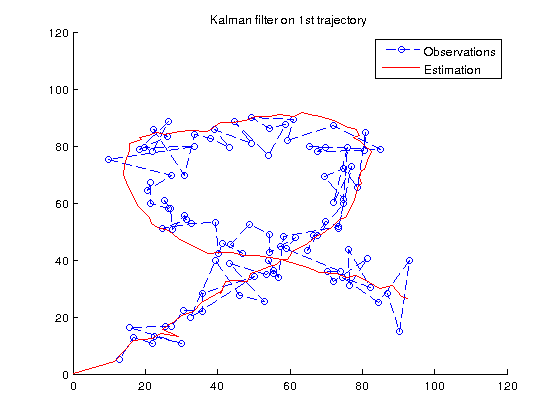
\includegraphics[width=15cm]{images/sigma01.png}
	\caption{Influence of $sigma$ on the filtered estimations. $\sigma^2=\frac{1}{100}$.}
	\label{fig:4}
\end{figure}

\begin{figure}
	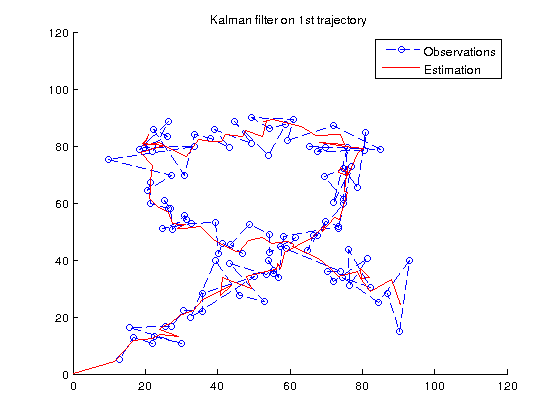
\includegraphics[width=15cm]{images/sigma1.png}
	\caption{Influence of $sigma$ on the filtered estimations. $\sigma^2=1$.}
	\label{fig:5}
\end{figure}

\begin{figure}
	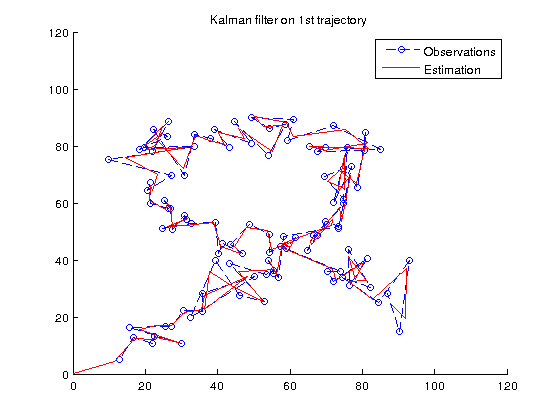
\includegraphics[width=15cm]{images/sigma10.png}
	\caption{Influence of $sigma$ on the filtered estimations. $\sigma^2=100$.}
	\label{fig:6}
\end{figure}

\paragraph{Improving filtering results}

In order to improve the filtering results, one has to decrease the observation noise. 
Since the observations are specified by equation \eqref{eqn:2} and we have $2$ independent observation trajectories, we can achieve this goal by calculating their average.
This cuts the variance of the observation noise by the factor 2, hence improving the accuracy of the filtering results.

\begin{eqnarray}
	Var \left( \frac{1}{2}(\pmb{Y}_k+\pmb{Y}^{\prime}_k) \right)&=& \Psi\pmb{X}_k + Var \left( \frac{1}{2} (\pmb{V}_k + \pmb{V}^{\prime}_k )\right)\\
	&=& \Psi\pmb{X}_k + \frac{1}{2} Var\left(\pmb{V}_k \right)
\end{eqnarray}
The last equation follows from the fact that $\pmb{V}_k$ and $\pmb{V}^{\prime}_k$ are decorrelated and thus independent.

\end{document}
